\section{Mapas}

\texto

\subsection{Altitude}

\begin{figure}[h!]
\centering
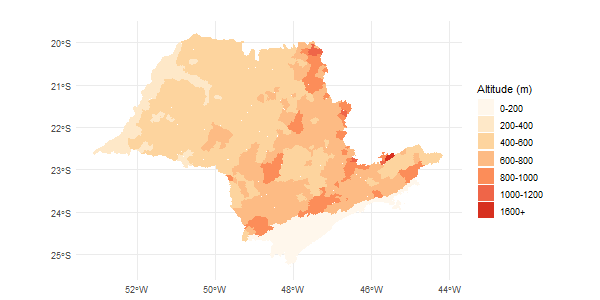
\includegraphics[height = 5cm]{Imagens/511.png}
\\{\scriptsize Figura 22. Distribuição espacial dos municípios do estado de São Paulo em classes segundo a altitude (m) de sua sede.}
\end{figure}

\texto

\subsection {Área}

\begin{figure}[h!]
\centering
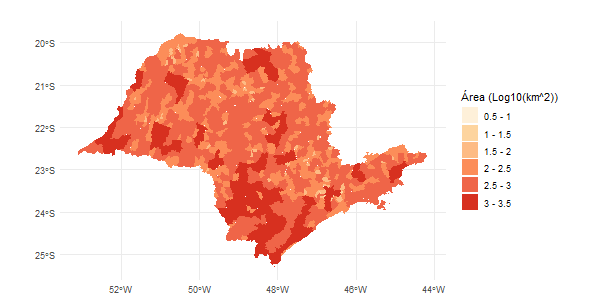
\includegraphics[height = 5cm]{Imagens/521.png}
\\{\scriptsize Figura 23. Distribuição espacial dos municípios do estado de São Paulo em classes segundo a área (Log10 km2).}
\end{figure}

\texto


\subsection {População}

\begin{figure}[h!]
\centering
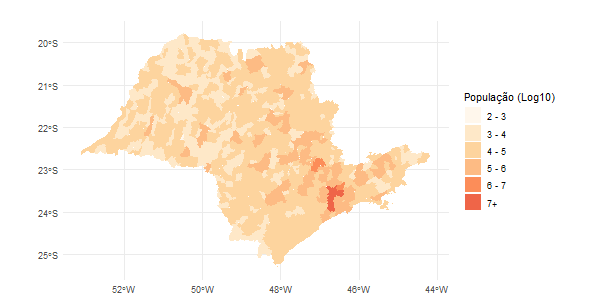
\includegraphics[height = 5cm]{Imagens/531.png}
\\{\scriptsize Figura 24. Distribuição espacial dos municípios do estado de São Paulo em classes segundo o tamanho da população humana (Log10 indivíduos).}
\end{figure}

\texto

\newpage

\subsection {Registros}

\begin{figure}[h!]
\centering
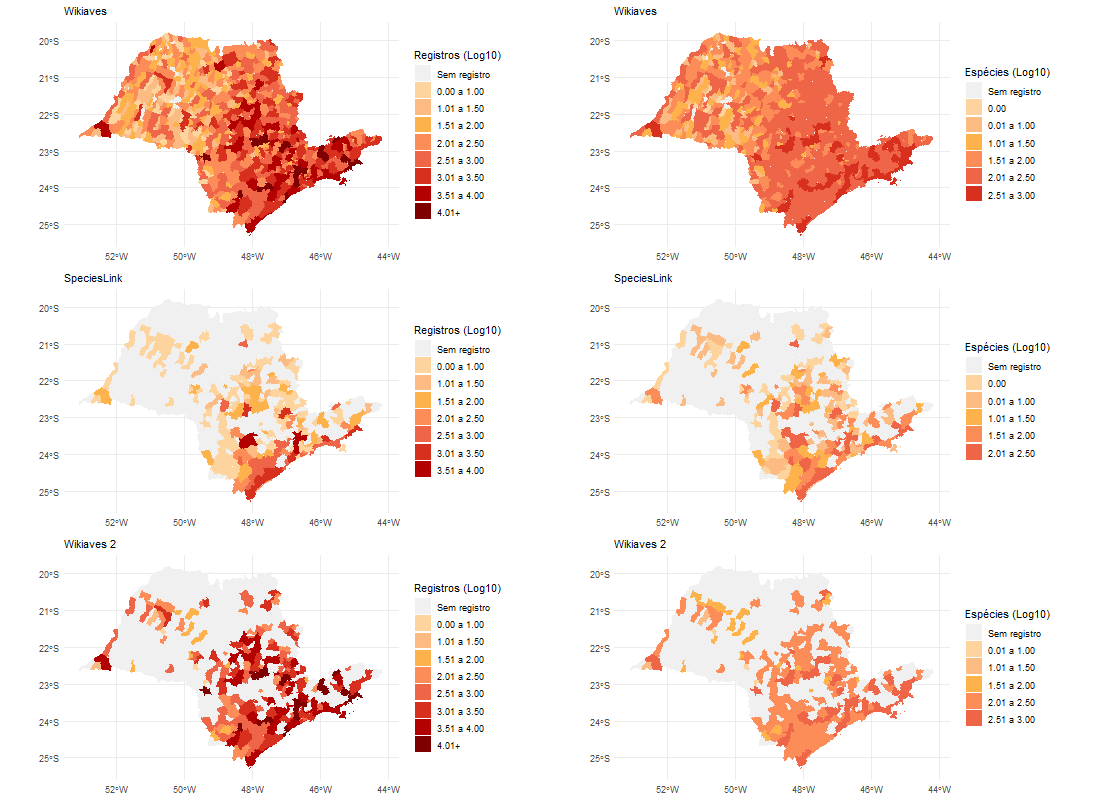
\includegraphics[width=17cm]{Imagens/561.png}
\\{\scriptsize Figura 25. Distribuição espacial dos municípios do estado de São Paulo em classes segundo o número de registros (Log10, esquerda) e o número de espécies (Log10, direita) em cada banco de dados (WAV = superior, SLI = central, WAV2 = inferior).}
\end{figure}

\texto

\subsection {Espécies}

\texto

